%------------------------------------------------------------------------------------
%	CHAPTER 4
%------------------------------------------------------------------------------------
\chapterimage{headerCap.jpeg}
\chapter{Registradores de 64 Bits}

\begin{remark}
	Dê o poder ao homem, e descobrirá quem realmente ele é. (Maquiavel - Diplomata, Autor e Historiador Italiano) 
\end{remark}

\section{Programa 5.1 - Retornamos ao Hello World}\index{Registradores de 64 Bits}
Podemos pensar o seguinte, até o momento para compilar nossos programas usamos 64 Bits, na instrução "nasm -f elf64", e isso é uma grande verdade, porém nossos registradores são todos de 32 bits, e isso causa um problema, pois não vimos nada de, por exemplo PILHAS, pois só funcionam em registradores de 64 bits. Assim devemos aprender a usá-los e a usufruir de seus benefícios.

Vamos lembrar da nossa tabela exposta no primeiro capítulo desse livro:
\begin{table}[H]
	\centering 
	\begin{tabular}{c | c | l }
		\textbf{64 bits} & \textbf{32 bits} & \textbf{Utilização} \\ \hline
		rax & eax & Valores que são retornados dos comandos em um registrador \\
		rbx & ebx & Registrador preservado. Cuidado ao utilizá-lo \\
		rcx & ecx & Uso livre como por exemplo contador \\
		rdx & edx & Uso livre em alguns comandos \\
		rsp & esp & Ponteiro de uma pilha \\
		rbp & ebp & Registrador preservado. Algumas vezes armazena ponteiros de pilhas \\
		rdi & edi & Na passagem de argumentos, contém a quantidade desses \\
		rsi & esi & Na passagem de argumentos, contém os argumentos em si \\
	\end{tabular}
\end{table}

A primeira coluna contém os registradores que veremos neste capítulo, a mudança básica é simples trocamos a letra "E" pela letra "R". No arquivo \textbf{makefile} já visto não precisaremos trocar uma única linha e por enquanto não usaremos nenhuma biblioteca, vamos começar limpos e entender quais são as mudanças necessárias. Começamos por criar um arquivo chamado \textbf{lerarquivo.asm} com a seguinte codificação:
\begin{lstlisting}[]
section .data
  mensagem: db "Hello World 64 bits!!!", 0xA
  tam: equ $- mensagem

section .text

global _start:

_start:
\end{lstlisting}	

Até o presente momento nenhuma mudança no nosso código (os dois pontos é um mero preciosismo da minha parte), porém:
\begin{lstlisting}[]
  mov rax, 0x1
  mov rdi, 0x1
  mov rsi, mensagem
  mov rdx, 0x17
  syscall
\end{lstlisting}

Agora começamos a verdadeira mudança, se bem lembramos a sequencia seria EAX, EBX, ECX e EDX, porém dois registradores são trocados, EAX muda realmente para RAX mas se reparou bem seu valor agora não é "0x4" como era, EBX agora vai mudar para RDI (e não RBX) e ECX para RSI (e não RCX como seria de se esperar) e finalmente RDX para RDX (como seria de se esperar). Além disso tudo, aparece a instrução "syscall" que procede a chamada do antigo "int 0x80".

Agora vamos as diferenças para encerrar o programa:
\begin{lstlisting}[]
  mov rax, 0x3C
  xor rdi, rdi
  syscall
\end{lstlisting}	

A primeira instrução uma simples mudança no endereçamento no qual ao invés de "0x1" agora usamos o "0x3C", zeramos o segundo registrador mas dessa vez utilizamos o comando XOR e finalmente uma chamada a "syscall" que fará o serviço de entregar o bloco de instruções ao computador.

E ao compilar e executar teremos corretamente a mensagem aparecendo no terminal: \\
{\ttfamily Hello World 64 bits!!!}

Nosso makefile agora terá a seguinte codificação:
\begin{lstlisting}[]
NOME = mostrar

all: $(NOME).o
	ld -s -o $(NOME) $(NOME).o
	rm -rf *.o

%.o: %.asm
	nasm -f elf64 $<
\end{lstlisting}	

Esse exemplo conhecemos que não se trata então de uma simples mudança de registradores mas quase reaprender novamente os comandos, mas não se preocupe apenas mantenha a mente afiada que veremos muito mais nesse capítulo.

\section{Programa 5.2 - Pilhas}\index{Registradores de 64 Bits}
Se o capítulo passado trouxe a sensação que agora vamos repetir todos os programas já vistos anteriormente, sinto em lhe dizer que está é totalmente errônea, porém sinta-se a vontade para refazê-los em 64 bits para treinar os novos registradores. Neste capítulo veremos do que são capazes, uma dessas mudanças é o conceito de \textbf{Pilhas}.

Não consigo compreender a confusão que faz com o iniciante a respeito desse assunto. Imaginemos uma pilha de caixas (uma sobre a outra), pensemos em umas 10, agora precisamos de uma para colocar algumas coisas, é óbvio que vamos pegar a última que colocamos (ou seja a que está em cima da pilha e não a primeira lá embaixo ou qualquer uma do meio nos arriscando a derrubar toda pilha), por isso mesmo \textbf{Pilhas} são conhecidas como LIFO (\textit{Last in First Out}), ou seja, a última que entrou na pilha será primeira a ser retirada.

Vamos começar nosso programa com a definição dos registradores:
\begin{lstlisting}[]
section .data
  LF            equ 10  ; Line Feed
  NULL          equ 0   ; Final da String
  EXIT_SUCESS   equ 0   ; Operação com Sucesso
  SYS_EXIT      equ 60  ; Codigo de chamada para finalizar

  STDIN         equ 0   ; System.in
  STDOUT        equ 1   ; System.out
  STDERR        equ 2   ; System.err

  SYS_READ      equ 0   ; read
  SYS_WRITE     equ 1   ; print

  liv1          db '1. Moby Dick', LF, NULL
  liv2          db '2. Tom Swayer', LF, NULL  
  liv3          db '3. Duna', LF, NULL
\end{lstlisting}

Apenas definimos os valores para nossos registradores e devemos observar os marcadores: liv1, liv2 e liv3 são eles que colocaremos na nossa pilha. O escopo principal do nosso programa:
\begin{lstlisting}[]
section .text

global _start

_start:
  ; Colocar os livros na pilha
  push      liv1
  push      liv2
  push      liv3
  ; Pegar um livro da pilha
  pop       rdi
  call      _imprimir
  pop       rdi
  call      _imprimir
  pop       rdi
  call      _imprimir
  ; Finalizar
  mov       rax, SYS_EXIT
  xor 		rdi, rdi ; Zerar
  syscall
\end{lstlisting}

Temos dois comandos novos: \textbf{PUSH} e \textbf{POP}, o primeiro deles insere um dado na pilha enquanto que o segundo obtém esse dado, sempre através do registrador \textbf{RDI}, ou seja o dado entra na pilha e saí pelo registrador \textbf{RDI}. Vamos para a função de impressão do dado:
\begin{lstlisting}[]
_imprimir:
  call  _ctCaracteres
  mov   rax, SYS_WRITE
  mov   rsi, rdi
  mov   rdi, STDOUT
  syscall
  ret
\end{lstlisting}

Devemos lembrar que para mostrar algo na saída precisamos ter conhecimento de seu tamanho, isso será realizado pela próxima função, aqui apenas fazemos o mesmo do programa anterior, movendo os registradores RAX (0x1), RSI (primeiro pois RDI contém o elemento da pilha) e RDI com seu valor de saída (0x1). E verificamos quantos caracteres temos no elemento de saída:
\begin{lstlisting}[]
_ctCaracteres:
  mov   rbx, rdi
  mov   rdx, 0
fazLoop:
  cmp   byte[rbx], NULL
  je    termina
  inc   rdx
  inc   rbx
  jmp   fazLoop
termina:
  ret 
\end{lstlisting}

Já vimos isso no passado, para contarmos os caracteres simplesmente a cada carácter não nulo incrementamos o valor de um registrador (neste caso RDX). E está tudo pronto e teremos como resposta ao executar este programa os livros colocados na pilha porém em ordem inversa: \\
{\ttfamily 3. Duna} \\
{\ttfamily 2. Tom Swayer} \\
{\ttfamily 1. Moby Dick}

Este é um conceito extremamente importante na programação, pois podemos organizar melhor a nossa informação.

\section{Programa 5.3 - Ler Arquivos}\index{Registradores de 64 Bits}
A leitura de arquivos com registradores de 64 bits é feito de forma semelhante aos de 32 bits, a diferença são os valores que passamos aos registradores. 

\begin{lstlisting}[]
section .data
  LF          equ 10 ; Line Feed
  NULL        equ 0  ; Final de uma string
  EXIT_SUCESS equ 0  ; Operação com Sucesso
  SYS_EXIT    equ 60 ; Código de chamada para finalizar

  STDIN       equ 0  ; System.in
  STDOUT      equ 1  ; System.out
  STDERR      equ 2  ; System.err

  SYS_READ    equ 0  ; leitura
  SYS_WRITE   equ 1  ; escrita / saída

  OPEN_READ   equ 0  ; abrir arquivo em modo leitura

  READ_FILE   equ 0  ; leitura do arquivo
  OPEN_FILE   equ 2  ; abrir arquivo
  CLOSE_FILE  equ 3  ; fechar arquivo

  file    db  'arquivo.txt', NULL
  tam_arq: equ 1024   ; 1 Kb Leitura

section .bss
  fd: resb    4 ; File Descriptor
  buffer: resb 4096    

section .text

global _start

_start:
\end{lstlisting}

Vamos começar com a criação das nossas constantes na seção Data, vou apenas repetir todas as que foram criadas e ampliar para as novas necessárias, que são:
\begin{itemize}
\item OPEN\_READ: colocar o arquivo em modo de obter os dados
\item READ\_FILE: ler os dados do arquivo
\item OPEN\_FILE: para realizar a abertura em modo leitura do arquivo
\item CLOSE\_FILE: fechar e encerrar o arquivo
\end{itemize}

Além dessas mais uma indicando o nome do arquivo e o tamanho de leitura desse. Já na seção BSS criamos uma variável para armazenar a posição de leitura do arquivo (\textit{File Descriptor}) e o buffer de leitura para o arquivo. Para abrir o arquivo:
\begin{lstlisting}[]
  mov rax, OPEN_FILE
  mov rdi, file
  mov rsi, OPEN_READ
  syscall
\end{lstlisting}

Abrimos o arquivo para leitura, indicamos qual arquivo será lido e colocamos este em modo de obtenção de dados. Bem semelhante ao que vimos para 32 bits. Para ler o conteúdo do arquivo:
\begin{lstlisting}[]
  mov [fd], rax ; armazenar o valor do File Descriptor
  mov rax, READ_FILE;
  mov rdi, [fd]
  mov rsi, buffer
  mov rdx, tam_arq
  syscall
\end{lstlisting}

Antes de qualquer ação armazenamos o conteúdo do \textit{File Descriptor} (obtido por RAX na abertura do arquivo), indicamos que o processo será leitura do arquivo, qual endereço do arquivo (\textit{File Descriptor}), aonde deve ser armazenada as informações e a quantidade de bytes buscada. Próximo passo é colocar o conteúdo em tela:
\begin{lstlisting}[]
  mov rax, SYS_WRITE
  mov rdi, STDOUT
  mov rsi, buffer
  mov rdx, tam_arq
  syscall
\end{lstlisting}

Indicamos que o processo será escrita, o local que deverá escrever (em tela), o quê deve escrever e a quantidade de bytes a serem escritos. E agora processamos o fechamento:
\begin{lstlisting}[]
  mov rax, CLOSE_FILE
  mov rdi, [fd]
  syscall

  mov rax, SYS_EXIT
  xor rdi, rdi ; Zerar
  syscall
\end{lstlisting}

Temos basicamente 2 passos para realizar em cada ação, no primeiro indicamos a ação de fechamento do arquivo e passamos o \textit{File Descriptor} e no segundo enviamos a ação de encerrar o programa e zeramos o registrador RDI.

Para testar o programa, certifique-se que na mesma pasta existe um arquivo em formato texto com o nome "Arquivo.txt".

\section{Programa 5.4 - Gravar Arquivos}\index{Registradores de 64 Bits}
A gravação de arquivos em 64 bits é uma operação que exige alguns conhecimentos específicos. Primeiramente, é necessário definir os valores adequados para a criação do arquivo, bem como para a sua abertura para gravação. É importante destacar que esses são dois processos distintos, e que é preciso ter cuidado ao executá-los.

Uma abordagem comum para lidar com essa questão é tentar realizar a criação do arquivo e, caso ocorra algum erro, executar o processo de abertura para gravação. Dessa forma, é possível contornar possíveis problemas e garantir que o arquivo seja criado e gravado corretamente.

É importante ressaltar que a gravação de arquivos em 64 bits pode ser uma tarefa complexa e que requer atenção aos detalhes. Portanto, é recomendável que se tenha um bom entendimento das especificações técnicas envolvidas antes de realizar essa operação. Que pode ser descrito conforme o seguinte fluxograma:
\begin{figure}[H]
	\centering
	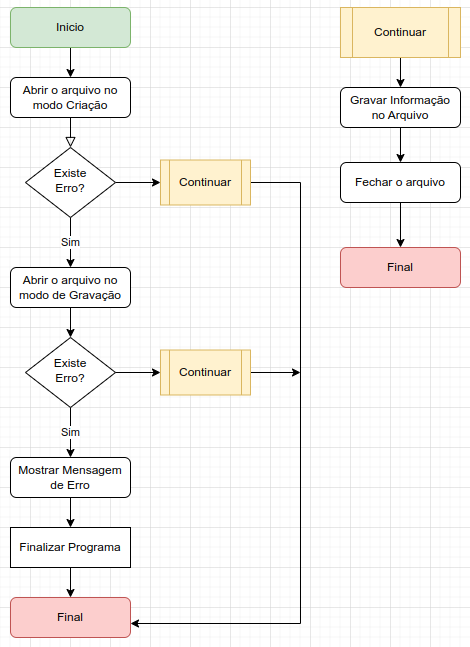
\includegraphics[width=0.5\textwidth]{Pictures/cap05/programa54}
	\caption{Fluxograma do Programa \textbf{Gravação de Arquivos}}
\end{figure}

Vamos começar com a definição das variáveis necessárias e tentar abrir o arquivo:
\begin{lstlisting}[]
section .data
    nomArquivo db 'arquivo.txt', 0x0
    conteudo db 'Hello World 2!', 0xA
    mens_erro db 'Erro ao abrir o arquivo!', 0x0

section .text
    global _start

_start:
    ; Abrir o arquivo
    mov rax, 0x2  
    mov rdi, nomArquivo
    mov rsi, 0x2 | 0x40 | 0x80 
    mov rdx, 0o666
    syscall
\end{lstlisting}

Vamos começar nosso programa e tentar criar o arquivo, que pode já existir, os códigos do registrador RSI são: 0x2 que corresponde a Leitura e Gravação; 0x40 para criação do arquivo e 0x80 que informa um erro caso a operação não seja efetuada. Para capturar o erro:
\begin{lstlisting}[]
    cmp rax, 0x0
    jl erroExiste
\end{lstlisting}

Comparamos se o retorno do registrador RAX for menor que zero saltamos para um ponto que tentará realizar outra forma. Caso contrário continuamos:
\begin{lstlisting}[]
continuar:
    mov rdi, rax
    mov rax, 0x1
    mov rsi, conteudo
    mov rdx, 15
    syscall
\end{lstlisting}

Apenas procedemos a gravação do conteúdo. Por fim fechamos este:
\begin{lstlisting}[]
    mov rax, 0x3
    mov rdi, [rsp]
    syscall
    jmp finalizar
\end{lstlisting}

Como estamos trabalhando com 64 bits não precisamos nos preocupar em guardar o File Descriptor pois o código do arquivo está guardado no topo da pilha, assim simplesmente o fechamos. Próximo passo é criar o ponto que será executado caso der erro no procedimento de gravação:
\begin{lstlisting}[]
erroExiste:
    mov rax, 0x2  
    mov rdi, nomArquivo
    mov rsi, 0x2 | 0x8 | 0x80 
    mov rdx, 0o666
    syscall    
\end{lstlisting}

Neste caso tentamos apenas abrir o arquivo para gravação, usando os códigos: 0x2 para abrir o arquivo em modo leitura/gravação; 0x8 para adicionar informação no arquivo e 0x80 que informa um erro caso a operação não seja efetuada.
\begin{lstlisting}[]
    cmp rax, 0x0
    jl erro
    jmp continuar
\end{lstlisting}

Novamente comparamos o registrador RAX com um valor menor que 0, se isso ocorre aconteceu algum problema que não é possível gerar o arquivo, caso contrário retornamos para a marcação \textbf{continuar} que procede a gravação e o fechamento do arquivo.
\begin{lstlisting}[]
erro:
    mov rax, 0x1
    mov rdi, 0x1
    mov rsi, mens_erro
    mov rdx, 25
    syscall
\end{lstlisting}

Caso ocorra a "pior" situação mostramos uma mensagem de erro, e por fim:
\begin{lstlisting}[]
finalizar:
    mov rax, 0x3C
    xor rdi, rdi
    syscall
\end{lstlisting}

Por fim finalizamos nosso programa. Ao executá-lo se o arquivo não existir será criado, e caso já exista a mensagem será colocada nele.
% Final do Capítulo
\clearpage